\documentclass[journal]{IEEEtran}

\usepackage[T1]{fontenc}
\usepackage[utf8]{inputenc}
\usepackage{graphicx}
\usepackage{booktabs}
\usepackage{amsmath}
\usepackage{array}
\usepackage{url}
\usepackage[hidelinks]{hyperref}

\begin{document}

\title{Checkable Properties for a Research Record:\\
A Specification, a Reference Validator, and Three Defects\\
It Found That Careful Reading Did Not}

\author{Andrew~H.~Bond%
\thanks{A. H. Bond is with the Department of Computer Engineering, San Jos\'e
State University, San Jos\'e, CA 95192 USA (e-mail: andrew.bond@sjsu.edu).}%
\thanks{Specification, validator, and both conformance reports are public at
\url{https://github.com/ahb-sjsu/philosophy-engineering}.}}

\markboth{IEEE Transactions on Technology and Society}%
{Bond: Checkable Properties for a Research Record}

\maketitle

\begin{abstract}
Research integrity rests on claims a reader is asked to take on trust. A paper
asserts that its hypotheses preceded its measurements, that nothing was omitted,
and that its conclusions do not outrun its evidence, and none of these assertions
is checkable from the artifact that makes them. We specify four properties of a
version-controlled research record that convert those assertions into predicates
a machine can refuse, implement a reference validator, and run it against two
live corpora. The validator found three classes of defect that accurate prose had
absorbed silently. Ordinary version-control hygiene destroyed the evidence for
twelve priority claims without anyone noticing, which forced a change to the
specification. A correction was propagated so completely that the published book
reads as though the stronger claim had never been made, leaving a blast radius of
zero that is the finding rather than the absence of one. Three results were
graded as requiring no modeling assumptions while their own dependency lists
named them. The validator also returned a result against the specification that
defines it: it was certifying the coherence level for a deployment whose
dependency graph its parser cannot populate, so that check was deciding an empty
graph. The same programme requires judgment procedures to prove they are not
vacuous, and the record specification carried no equivalent condition. It now
does, and the reference deployment moves down a level as a result: what it
demonstrated was never coherence, only the absence of anything to be incoherent
about. Converting that deployment to a format with a dependency field then
surfaced a second gap, larger than the first. The specification gives claims a
priority property and gave dependency edges none, so a graph wired after its
results are known could not be told from one declared in advance. We wired one
that way and the checker accepted it, so we added the missing property: edges
now carry provenance, and blast radius is reported over the subgraph whose
declarations can be shown to predate their results as well as over the whole.
Measured that way the two deployments stand at 0.25 and 0.00.
\end{abstract}

\begin{IEEEkeywords}
Research integrity, reproducibility, preregistration, provenance, scientific
record, audit, accountability, research software.
\end{IEEEkeywords}

\section{Introduction}

\IEEEPARstart{A}{research} paper makes claims about the world and claims about
itself. The first kind is scrutinized. The second kind is not, because it cannot
be. When a paper states that its hypotheses were fixed before the data were seen,
that no analyses were run and discarded, and that its conclusions are supported by
the evidence cited, a reader has no way to test any of it from the artifact in
front of them. These are assertions about an unobservable process, made by the
only party with an interest in the answer.

Reform has concentrated on external registries, which work and which we build
on. Preregistration establishes priority through a trusted third party.
Registered reports make it a condition of publication. Both operate on the study
as a unit. Neither addresses what happens afterwards, inside a body of work, when
one result fails and the author must determine what else falls.

Four difficulties survive that reform, and all four are structural rather than
cultural. The unit of publication is the paper while the unit of truth is the
claim, so a paper with nine sound results and one bad lemma has no way to
express that state. Because the artifact is indivisible, correcting the lemma
means retracting everything bundled with it, which makes correcting nothing the
rational choice. Nothing records what depended on the lemma, so the question of
what else falls is answered from memory. And the absence of a result is invisible
by construction, which makes any claim to have reported everything a claim about
a set no one can inspect.

This paper reports an attempt to make those four assertions checkable. We
specify four properties of a research record held in version control, implement a
validator that decides them, and run it against two corpora that were not built
for it. Our contribution is not the components. Claim-level publication,
argumentation graphs over evidence, and version-controlled manuscripts all
predate this work by a decade or more, and Section~\ref{sec:related} says so at
length. The contribution is the conjunction, operated against live corpora, and
the measurements that follow.

Three results are worth stating in advance. First, the checks found defects that
careful reading had not, and the defects were of a kind prose cannot hold rather
than a kind the authors were careless about. In one corpus, ordinary rebasing
destroyed the evidence for twelve priority claims while the written record
remained accurate throughout. Second, one class of accountability failure appears
to be undetectable by any existing mechanism: a correction can be propagated so
thoroughly that no trace of the retired claim survives, which leaves a published
work reading as though it had never erred. We recover it only because an
append-only record holds the claim and its withdrawal at the same time. Third,
running the validator against our own specification exposed a gap in the
specification. It certifies the coherence level for a deployment whose dependency
graph is empty, because the parser for that deployment's format cannot represent
dependency edges. A sibling part of the same programme requires judgment
procedures to demonstrate that they are not vacuously compliant, and the record
specification has no matching requirement.

\section{Four Properties}
\label{sec:properties}

The record is a set of claim objects in a git repository. Each carries an
identifier, a statement, an evidence class, declared dependencies on other
claims, and where applicable a registration sealed before measurement. Classes
are ordered by the support they assert, from \texttt{exploratory} through
\texttt{demonstrated} and \texttt{replicated} to \texttt{proved}, with
\texttt{withdrawn} and \texttt{refuted} for claims that have lost support. The
four properties are predicates over that structure.

\begin{table}[!t]
\caption{The four properties. Each converts an assertion normally taken on trust
into a predicate over a version-controlled record.}
\label{tab:props}
\centering
\footnotesize
\begin{tabular}{@{}p{0.055\columnwidth}p{0.36\columnwidth}p{0.47\columnwidth}@{}}
\toprule
& \textbf{The assertion} & \textbf{The predicate} \\
\midrule
P1 & We registered before we measured & The sealing commit is a git ancestor of the first commit adding the result \\
P2 & There is no file drawer & The identifier sequence is gap-free and every identifier resolves to a disposition \\
P3 & We do not assert beyond our evidence & No narrative document cites a claim above its class \\
P4 & We know what depends on what & Every declared dependency resolves, and no claim outranks its weakest support \\
\bottomrule
\end{tabular}
\end{table}

\textbf{P1 uses repository ancestry rather than a timestamp.} A third-party
registry proves wall-clock time and requires trusting the registry.
\texttt{git merge-base -{}-is-ancestor} proves order and requires trusting
nothing, but is checkable by anyone holding a copy of the repository.
Section~\ref{sec:greenfield} reports what this choice costs.

\textbf{P2 is the property we would defend first.} No file drawer is ordinarily
an unfalsifiable claim, since it quantifies over work that was never recorded.
Requiring identifiers to be assigned contiguously, and requiring every
identifier to carry a disposition including the abandoned and the never-run,
converts it into a property of a finite list. A programme hiding a failed run
under this regime must either leave a visible gap or write a false disposition.
The guarantee is bounded by where the identifier space begins, which
Section~\ref{sec:limits} treats as the limitation it is.

\textbf{P4 makes the consequences of a refutation computable.} When a claim
fails, the set of claims resting on it is obtained by traversing declared edges
rather than by recollection. We call the result the blast radius. The design
intent is that a bad result prunes a branch instead of burning the tree, and
Section~\ref{sec:brownfield} measures whether it does.

Conformance is layered. L1 requires the objects and P2. L2 adds P1. L3 adds
declared dependency edges, P4, P3, and blast-radius reporting. L4 additionally
requires fresh-context verification records and machine-checked cores as linked
objects. L1 is achievable by one researcher in an afternoon and already delivers
the file-drawer guarantee.

\section{The Validator}

\texttt{pe\_lint.py} is 939 lines of Python with no dependencies outside the
standard library and \texttt{git}. It parses two record formats, decides P1
through P4, computes blast radius, and exits non-zero when the requested level is
not met, which makes it usable as a continuous-integration gate.

Two design choices are worth reporting because both were forced by deployment.

\textbf{The ratchet.} A conversion of an existing corpus surfaces
contradictions that the converter is forbidden to resolve, because resolving
them would mean rewriting the work rather than describing it. Left alone, these
hold the gate permanently red, and a gate that always fails gates nothing. The
validator therefore accepts a baseline of acknowledged findings, each naming an
owner and what would settle it. The mechanism is built so that it cannot be used
to launder claims. Entries match on exact finding text, so a promoted claim stops
matching and reappears. A stale entry fails the run. A missing owner fails the
run. No run with a non-empty baseline may report unconditional conformance, and
the report says so on its own output. A baseline may only shrink.

\textbf{Two front ends.} One deployment stores claims as native JSON objects.
The other predates the specification and stores them as markdown tables. The
markdown parser recovers identifiers, classes, statements, and registrations.
It does not recover dependency edges, because the format has no field for them.
Section~\ref{sec:selfcheck} reports what that costs, and it is the most serious
finding in this paper.

\section{Deployment A: a record built under the specification}
\label{sec:greenfield}

The first deployment is the evidence ledger of an observation-theory programme:
78 claims, and a registry of 91 sealed registrations.

Under the amended specification of Section~\ref{sec:selfcheck} it conforms at
L2, and the L3 it was previously reported at was vacuous. P2 holds over the full
range 001 to 091 with zero gaps and
four identifiers carrying no result: two never assigned and proven absent from
the full history, one reservation abandoned before sealing, and one burned by a
design failure that its own pilot caught. P4 reports no support-cap violations.
P3 scans three narrative documents and raises two warnings. Priority verifies on
all 32 seals that carry checkable anchors.

That clean report is the second one. The first run failed, and the failure is
the useful part.

\textbf{Twelve priority proofs had been destroyed by ordinary tooling.} One seal
resolved but failed ancestry. Eleven named commits that no longer existed. The
cause was the same in both cases and it was not misconduct: rebasing rewrites
commit hashes, and a recorded seal hash is a reference to an object that rebasing
destroys. The eleven were sealed during a period when the author was pushing from
several machines with rebase-on-pull. The priority was genuine in every case. The
evidence for it was collateral damage from routine version-control hygiene, and
the registry's own notes show the author had observed the rebase without
observing that it had broken the proof.

This forced a normative addition to the specification. A conforming record must
not rewrite history containing seal commits. Registrations must carry a content
hash independent of commit identity, so that a rewritten record can be
re-anchored. A rewritten seal must record the old-to-new mapping in its row. And
a non-resolving seal without such a mapping is a failure rather than a warning,
because a claim whose priority cannot be checked is a claim whose priority is
unproven.

Remediation recovered all twelve. The re-anchoring script refuses to write unless
the content hash still matches under the repository's own sealing scheme, the
commit is the first that added the registration file, and it is an ancestor of
the result commit. A pre-rebase hook now refuses any rebase touching the
registration directory. A separate script anchors the content hash to a
third-party timestamp, which closes the gap that ancestry leaves open: ancestry
proves order, and an anchor proves wall-clock time to a stranger.

\textbf{Remediation then found a third defect.} Two registrations failed the
content-hash check. Both carried dated, disclosed amendments appended to the
sealed body after sealing, which the protocol permits. Appending them changed the
body, so the seal hash stopped verifying. The specification had required
amendments to be dated and reasoned and had said nothing about their effect on
the content commitment. The correct design, now stated, is that the sealed body
is immutable and amendments are appended as separately hashed records.

None of these three defects was detectable by reading. The written record was
accurate throughout.

\section{Deployment B: converting an existing corpus}
\label{sec:brownfield}

The second deployment is a book of roughly thirty-five thousand lines with
associated papers, written over several years before the specification existed.
Conversion produced 236 claim objects. It is descriptive first: no claim was
re-derived, no statement was edited, and nothing was deleted, on the ground that
priority is the one property that no later rigor reconstructs.

The fraction of claims entered without a prior registration is 0.958. That number
is a measurement rather than a criticism, and near unity is expected by
construction for any corpus converted after the fact. What matters is its
trajectory.

\subsection{The blast-radius distribution}

The corpus declares 196 dependency edges, with 154 of 236 claims carrying at
least one. Fig.~\ref{fig:blast} shows the blast radius of every claim, computed
by traversal.

\begin{figure}[!t]
\centering
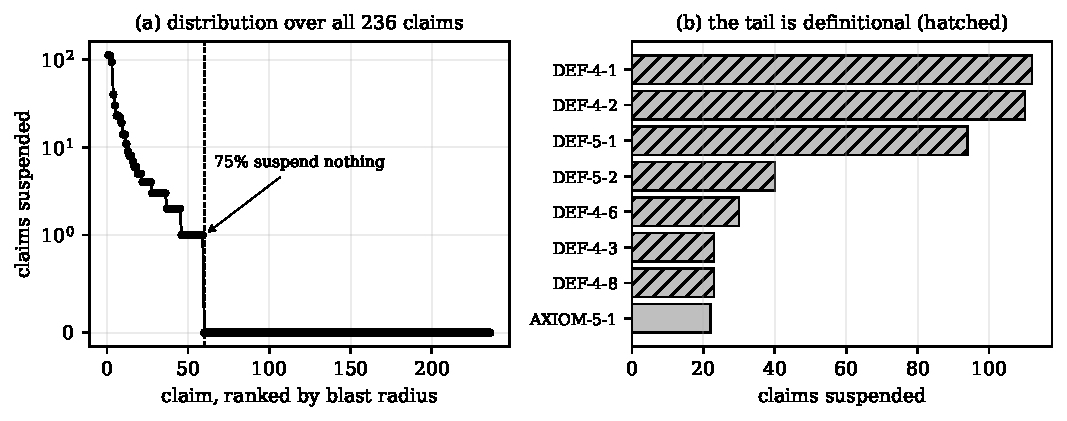
\includegraphics[width=\columnwidth]{build/fig_blast.pdf}
\caption{Blast radius of every claim in Deployment B, computed from the live
record. (a) The distribution is sharply right-skewed: 75.0\% of claims suspend
nothing at all and 84.8\% suspend two or fewer, while the largest suspends 112.
(b) The tail is definitional. The claims whose refutation would reach furthest
are the definitions of the underlying mathematical objects, not the empirical
results. A refutation in this corpus almost always prunes a branch; the
exceptions are foundational by construction.}
\label{fig:blast}
\end{figure}

Mean blast radius is 2.77 and the median is 0. The maximum in-degree is 33. The
shape is the one a theory of research programmes would predict, in which
refutations ordinarily strike auxiliary claims and leave a protected core
untouched, and the distribution locates that core in a particular place: the
seven claims with the largest blast radius are all definitions of the underlying
mathematical objects.

We flag an ambiguity rather than resolve it. A heavy tail concentrated on a few
high in-degree claims is consistent with a genuine foundational core, and it is
equally consistent with dependencies being under-declared everywhere else. This
corpus gives evidence for both readings. The conversion logged 29 claims whose
declared dependencies point outside the record entirely, and wired only 49 of 81
previously untagged results to their roots. The distribution in
Fig.~\ref{fig:blast} is therefore measured on a graph its own conversion report
describes as incomplete, and we draw no conclusion about research programmes in
general from a single partial graph.

\subsection{Two findings the checker made visible}

\textbf{A refutation that pruned five claims out of 140.} The corpus asserts a
symmetry group larger than the one its evidence supports. The measured result
supports a four-element group; a larger group is posited and would require an
operation that is nowhere measured. Suspending the over-strong claim suspends
five dependent theorems and leaves the rest untouched, and the report names both
sets explicitly. That is the intended behavior, and it is the difference between
pruning and burning.

\textbf{A correction with a blast radius of zero, which is the finding.} The
corpus had committed to a conservation law as a chapter thesis. The author later
judged the claim to overreach and retreated to a weaker statement about
invariance, giving the reason in a commit message. The work was careful: 87
occurrences rewritten, text nodes only, with all 2{,}126 equations verified
identical before and after. It was also complete. The current version contains
zero occurrences of the retired phrasing and 47 of the replacement.

That completeness is the problem. The published book now reads as though the
stronger claim was never made, and a reader cannot discover that a thesis was
retired, because every trace of it was correctly removed. The only surviving
record of the retreat was a commit message. Entered into the record as
\texttt{withdrawn}, the claim reports a blast radius of zero, and the zero is the
result: it is the formal statement that this correction was propagated perfectly
and recorded nowhere.

We think this is the most consequential finding in the paper for research
accountability, because no existing mechanism detects it. Retraction notices
address papers that are withdrawn. Version control records that text changed.
Neither surfaces a thesis that was quietly weakened and then made invisible by a
thorough edit. A programme that counted only suspensions would score this episode
as a non-event. The general statement is uncomfortable: a retraction thorough
enough to be invisible is indistinguishable from never having erred, and only an
append-only record holds the claim and its withdrawal at the same time.

\subsection{Contradictions only the author can settle}

Three results are graded as following from standard mathematics without modeling
assumptions, while their own dependency lists name modeling constructs. A result
cannot be both. Either the grade or the dependency list is wrong, and the
specification forbids the converter from deciding which. These are the record's
four surviving coherence errors, they are acknowledged in the baseline with a
named owner, and the current run reports conformance against that baseline while
stating on its own output that it is not unconditional. Four further claims raise
warnings for being classified as definitions while resting on substantive claims,
which the specification treats as a modeling assumption in disguise.

The conversion also found 81 numbered results carrying no epistemic grade and
appearing in no registry, roughly a third of the corpus's formal content, and
therefore invisible to the corpus's own accounting before conversion.

\section{What the validator found in the specification}
\label{sec:selfcheck}

The result with the most consequence here came from pointing the validator at
the specification that defines it. We report it the way we report the others,
because a check that returns something is a check doing its work, and a
specification that could not be caught by its own instrument would be the more
troubling object.

Deployment A is certified at L3. L3 requires declared dependency edges, P4, and
blast-radius reporting. Deployment A's record is stored as markdown tables, and
the markdown parser assigns no dependency edges, because the format has no field
for them. We verified this directly: zero of its 78 claims carry a dependency
edge, and the parsing routine never assigns the field. P4 therefore evaluates
over an empty graph, finds no violations because there is nothing to violate, and
reports PASS. Blast radius is zero for every claim in that deployment for the
same reason. The validator reports conformance at the level whose entire purpose
is dependency structure, for a record that declares none.

This is a vacuous-compliance failure, and it is a failure the same programme
already knows how to prevent. Elsewhere in this body of work, a judgment
procedure is required to be invariant under declared transformations, and that
requirement is paired with an explicit non-degeneracy condition, because a
constant function satisfies invariance perfectly and is useless. The record
specification imposes no analogous condition on its own dependency graph. It
demands non-degeneracy of the systems it governs and does not demand it of
itself.

The fix is straightforward to state. L3 should require dependency declaration to
be non-vacuous, by reporting edge coverage as a first-class statistic and
refusing to certify blast-radius conformance when the graph is empty or when
coverage falls below a declared threshold. A format that cannot express
dependency edges should be capped at L2 rather than certified at L3.

We implemented it. The specification gained a non-vacuity clause requiring that
edge coverage be reported in every run, that a ledger declaring no resolving
dependency edge fail, and that a storage format incapable of expressing such an
edge be capped at L2, where no property quantifies over the graph. A programme
may declare a minimum coverage and the validator enforces it; the specification
declines to set a general floor, because the defensible value depends on how many
of a corpus's claims are independent of the rest.

The effect on the two deployments is asymmetric. Deployment A now fails L3 and
conforms at L2. Nothing about that programme changed: its claims, its seals, and
its registry accounting are exactly as previously reported, and no scientific
result is affected. What changed is that the report no longer states that
coherence was verified when what was verified was an empty graph. Deployment B is
unaffected, declaring 196 resolving edges across 154 of its 236 claims, an edge
coverage of 0.653, and continuing to conform at L3 against its baseline.

The gap had persisted through a written conformance report and a published case
study without a reader noticing, which is the same pattern as the other three
findings and the reason we think the exercise is worth the cost. Readers checked
whether the coherence property passed. Deciding whether it had anything to pass
over is the kind of question a check answers cheaply and a reading does not
answer at all.

\section{Wiring a graph into Deployment A}
\label{sec:spine}

The non-vacuity clause caps a format that cannot express edges, which invites the
obvious response: give it one. Deployment A was converted to native claim
objects, 77 of them, one per ledger row.

Edges were produced as candidates mechanically, by finding every mention of one
claim's identifier inside another claim's row together with its surrounding
sentence, then adjudicated one at a time by reading that sentence. Type
assignment was not automated, because the specification is explicit that a
checker cannot separate an edge a claim rests on from a contextual one, and an
automated guess would have manufactured exactly the structure the exercise
measures. Fifty-two raw candidates reduced to twenty-five after excluding matches
inside a row's own identifier cell, and twenty-seven edges were declared: eight
bearing weight, three corroborating, sixteen contextual.

	extbf{Most of the first run was the converter's error, and reporting that is
part of the result.} The first run raised 44 errors, of which 43 were ours: every
object had been marked retrospective on the reasoning that its edges were written
today, which is the wrong object, since that flag is about a claim's own priority
and these claims are registered. The second run raised 12, of which 6 were ours:
the registration detector matched one of the ledger's naming schemes, and
reported the entire crucible family, sealed before any test ran under a different
scheme, as unregistered. A conversion run by someone less familiar with the
corpus would have recorded six false accusations of missing priority. The residue
after both corrections is six findings.

Three claims assert a class requiring prior registration while their rows name no
registration under any scheme. Two verification records carry a prediction class
where the specification provides record classes that carry no evidence grade of
their own. Two claims are tagged with a class token the specification does not
define, which the parser read as a live class where the programme means a
terminal one. A table header has been counted as a claim in every previous report
of this ledger, so the true count is 77 and not 78. And the two front ends are
exclusive, so no single invocation reads both the claim objects and the registry
accounting table.

The sixth is the one the graph was built to find. 	exttt{GO-12} is classed as
registered in advance and rests on 	exttt{GO-11}, which is not; under the
partial order over classes neither dominates the other, and the check refuses the
claim. The content is not bookkeeping. Priority does not propagate upward through
a dependency: a claim registered before its test, resting on a claim that was
not, cannot carry its registered standing past the joint. That is invisible in
prose, and it is what a declared graph is for.

\subsection{What the conversion showed about the specification}

Twenty-seven edges were declared into a corpus whose results were all in, and the
validator accepted every one without comment. The specification gives claims a
priority property and gives edges none. Nothing requires an edge to have been
declared before the test it bears on, nothing records when an edge was declared,
and no check separates a graph wired in advance from one wired afterwards.

This bears on the companion manuscript, which argues that a claim ledger makes a
research programme's core-and-belt partition a property of the record rather than
a reconstruction made by someone who already knows which commitments survived.
That argument needs the edges to be prospective. A ledger conforming at the
highest level defined today may have been wired entirely in hindsight, and this
one was. The companion now states its claim as what a ledger makes possible
rather than as what any deployment demonstrates.

The remedy has a precedent inside this programme. The discovery arm met the same
problem for transformation families and resolved it by admitting a late row only
when it carries the date it was written, names the sealed artifact holding the
real declaration, and shows that declaration preceding the result. Dependency
edges want the same three fields, and blast radius should then report the
prospective subgraph separately, since that is the only part of a graph the
appraisal argument is entitled to.

We implemented it. An edge entry may now carry the date its dependency was
declared, the date the row was written, and a pointer to the sealed artifact
holding the declaration; it classifies as prospective, backfilled, retrospective
or unrecorded; the checker refuses a backfill that names no declaration and one
entered before it was declared; and every run reports the four counts, the
prospective fraction, and blast radius over the prospective subgraph beside the
full one. Unrecorded edges are reported rather than failed, because requiring
provenance on every edge would make every converted corpus non-conforming at a
stroke, and a conversion nobody can enter is a conversion nobody performs.

Populating it was the test that mattered, and it was done from the record rather
than by assertion: each of the eight edges was audited by asking whether the
source claim's sealed registration already names the target. Two do. One of them
is the edge that produced the support-cap violation above, which means that
inconsistency is not an artifact of wiring the graph today. The programme
committed in advance to \texttt{GO-12} resting on \texttt{GO-11}, and the class
assignment has disagreed with that commitment ever since.

The two columns the mechanism produces are the ones the appraisal argument turns
on. Refuting \texttt{GO-11} strikes two claims on the programme's present
beliefs and one on what the record can show it fixed in advance. Deployment A's
prospective fraction is 0.25 and Deployment B's is 0.00, its 196 edges being
entirely unrecorded. Both remain as conforming as they were. What has changed is
that a programme can no longer report the full blast radius while claiming the
warrant of the prospective one, because the report prints both.

\section{Discussion}

The defects reported here fall into three classes, and the classes suggest what
this kind of checking is for.

The first class is identity loss under ordinary tooling. Twelve priority proofs
were destroyed by rebasing, in a repository whose written record was accurate
throughout, and no reader could have found it. This class is invisible to human
review because the thing that broke was a machine-checkable reference and not a
statement.

The second class is the complete and unrecorded correction. It is invisible for
the opposite reason: the work was done properly and the evidence of it was
removed as part of doing it properly. Only an append-only structure catches this,
and catching it requires the counterintuitive step of treating a blast radius of
zero as a result rather than as silence.

The third class is self-contradiction across distance. A result graded as
assumption-free while its own dependency list names assumptions, or a
falsification condition contradicted 112 lines later in the same file, is a
defect a reader can find only by holding two distant passages in mind at once.
Machines hold distant passages in mind cheaply.

What checking does not do is also worth stating. It cannot tell whether a claim
is true. It cannot propagate along dependencies nobody declared, which is the
classical point that no hypothesis is tested in isolation and the reason
undeclared edges are this method's blind spot. It cannot decide the two P3
warnings in Deployment A, because distinguishing a citation the claim rests on
from a contextual one requires knowing which the author intended, and the
markdown front end does not record it.

There is a governance problem that the technical work does not touch. Every
institution that made record-keeping stick had an outside party entitled to
inspect and to impose a cost: journals enforce registration, regulators enforce
trial registries, editors enforce review. A record operated by the only party it
constrains has no such enforcement, and the properties it checks are adopted
voluntarily by the person they restrain. Nothing in the specification fixes this,
and we think it is the most likely way for the method to fail in practice while
appearing to succeed on paper.

\section{Limitations and disclosed negatives}
\label{sec:limits}

Two corpora, both maintained by this paper's author, who chose the method and
then reported that it worked. The confirmation risk is severe and cannot be
reduced from inside. Nothing here has been tried by a programme with different
authorship, and the measurements in Fig.~\ref{fig:blast} should be read as one
observation rather than as a distribution over research programmes.

A companion set of checks, governing which transformations a claim was tested
against, does not pass on this programme. Ten tests cite three transformation
families that the relevant registry never declares. The families were declared in
the individual sealed registrations and were not mirrored into the registry.

That finding produced the second specification change reported in this paper, by
the same route as the first. The specification admitted only a conforming row or
a missing one, so a registry repaired after the fact was indistinguishable from a
registry whose families were chosen to fit results already seen. It now
distinguishes them. A late row is admissible as a backfill when it carries the
date it was written, names the sealed artifact holding the real declaration with
path, content hash, and sealing commit, and when that declaration demonstrably
precedes the result, which means the seal commit is an ancestor of the commit
adding the result and the sealed artifact still hashes to its recorded value.
Where the third condition cannot be shown the row must not be entered, and
deleting the offending tests is not a repair either, because removing the record
of a test that ran is the file drawer P2 exists to prevent. Backfilled rows are
reported rather than passed over, on the reasoning that a registry with many of
them belongs to a programme that is not writing declarations down when it makes
them.

We do not report whether the reference registry has since been repaired under
that clause. Those registries are not public, and this paper verifies only what
it can run.

P2's guarantee is narrower than its name. Contiguous identifiers make the set of
identified lines of work enumerable. They say nothing about work considered and
never given an identifier, and the boundary of the identifier space is set by the
same party the property is meant to constrain.

Deployment A does not claim L4. Fresh-context verification records and
machine-checked cores both exist in that programme, but they are recorded in
prose rather than as linked objects, and claiming a level whose requirement is
linked objects would be the error this apparatus exists to prevent.

Finally, Section~\ref{sec:selfcheck}'s clause left the two deployments incomparable on
coherence, and Deployment A has since been converted to a format with a
dependency field, reported in Section~\ref{sec:spine}. It now carries a real but
sparse graph at 0.078 edge coverage against Deployment B's 0.653, and the gap is
a fact about the corpora rather than about the checker: most of Deployment A's
dependency structure is not written down in any document a converter can read.

\section{Related Work}
\label{sec:related}

Preregistration establishes the norm P1 enforces, and registered reports make it
a publication condition, at a scale this work does not approach. The differences
are that registries are external services whose timestamps must be trusted, and
that registration is per-study rather than per-claim with a dependency graph.

Claim-level publication was proposed as nanopublications, in which the smallest
publishable unit is a single assertion with its provenance, and developed as
micropublications, which link claims to evidence and to each other with support
and challenge edges. Both predate this specification and both have better formal
serializations. They solve granularity and linkage. Neither makes the absence of
a claim observable, neither establishes that a prediction preceded its test, and
neither defines what a challenge does to the class of a dependent claim.

Manubot treats manuscripts as version-controlled repositories with continuous
integration, which is the infrastructure model assumed here; it versions the
document, and this work versions the claims inside it. Proof-assistant libraries
already compute blast radius exactly, for the fragment of claims that can be
formalized, and are the closest existing system to the ideal. The contribution
here is an attempt to extend that discipline to empirical claims, where no
compiler exists and edges must be declared by hand.

Lakat proposes a peer-to-peer architecture for continuous-integration publishing
with a review-based consensus mechanism. Its concern is the governance of a
distributed publishing system rather than the appraisal of a single programme's
record. The broader reform movement in psychology reached the conclusion that
changes of this kind are reform of evidentiary standards rather than changes of
theory, and we agree.

We do not offer a better registry, a better claim format, or a better proof
assistant. We offer the conjunction, and the measurement of what it caught.

\section{Conclusion}

Four assertions that research artifacts normally make on trust can be stated as
predicates over a version-controlled record, and a 939-line checker can decide
them. Run against two corpora that were not built for it, the checker found
priority evidence destroyed by routine tooling, a correction so complete that it
erased the record of its own occurrence, and results graded above the support
their own dependency lists declare. None of the three was visible to careful
reading, and the written record was accurate in every case.

The checker also found that our specification certifies its coherence level for a
record with no dependency graph, which is the vacuous-compliance failure that the
same programme requires the systems it governs to rule out. We have stated the
fix and left it unapplied, because it changes the standing of a deployed record
and that decision belongs to the specification's owner.

The property we would defend first is the second one. No file drawer is normally
a claim about a set nobody can inspect. Assign identifiers contiguously, require
every identifier to carry a disposition including the abandoned and the
never-run, and it becomes a property of a finite list that anyone can check in
seconds. That conversion, from an unfalsifiable assurance to a finite check, is
what the rest of this apparatus is for.

\section*{Companion Paper}

The question of why these four properties and not others is a question about the
appraisal of research programmes, and it is treated separately in a companion
manuscript that carries no empirical content. That paper argues that declaring a
dependency partition before a test, and proving priority by repository ancestry,
converts a distinction that philosophy of science could previously draw only in
hindsight into a property of the record. The two papers are separable: this one
reports what a checker found and stands without the argument, and the companion
makes an argument and states explicitly that it has no measurements. The
blast-radius distribution in Fig.~\ref{fig:blast} is the first test of a
prediction that companion states.

\section*{Acknowledgment of AI Use}

Drafting, prior-art search, figure construction, and structural editing were
performed with the assistance of a large language model under the author's
direction. Every quantity reported here was produced by the scripts in the
repository's \texttt{build} directory, reading the live records, rather than
transcribed. The author is responsible for the claims and the verdicts.

\begin{thebibliography}{99}
\footnotesize

\bibitem{chambers}
C.~D. Chambers, ``Registered reports: A new publishing initiative at
\emph{Cortex},'' \emph{Cortex}, vol.~49, no.~3, pp.~609--610, 2013.

\bibitem{groth}
P.~Groth, A.~Gibson, and J.~Velterop, ``The anatomy of a nanopublication,''
\emph{Information Services and Use}, vol.~30, no.~1--2, pp.~51--56, 2010.

\bibitem{clark}
T.~Clark, P.~N. Ciccarese, and C.~A. Goble, ``Micropublications: A semantic model
for claims, evidence, arguments and annotations in biomedical communications,''
\emph{Journal of Biomedical Semantics}, vol.~5, art.~28, 2014.

\bibitem{manubot}
D.~S. Himmelstein \emph{et al.}, ``Open collaborative writing with Manubot,''
\emph{PLOS Computational Biology}, vol.~15, no.~6, e1007128, 2019.

\bibitem{ioannidis}
J.~P.~A. Ioannidis, ``Why most published research findings are false,''
\emph{PLoS Medicine}, vol.~2, no.~8, e124, 2005.

\bibitem{merton}
R.~K. Merton, ``The normative structure of science,'' in \emph{The Sociology of
Science: Theoretical and Empirical Investigations}. Chicago, IL, USA: Univ. of
Chicago Press, 1973, pp.~267--278. % verify: orig. 1942, reprinted here

\bibitem{lakat}
L.~Horstmeyer, ``Lakat: An open and permissionless architecture for continuous
integration academic publishing,'' arXiv:2306.09298, 2023.

\bibitem{vazire}
S.~Vazire, ``Implications of the credibility revolution for productivity,
creativity, and progress,'' \emph{Perspectives on Psychological Science},
vol.~13, no.~4, pp.~411--417, 2018.

\bibitem{haber}
S.~Haber and W.~S. Stornetta, ``How to time-stamp a digital document,''
\emph{Journal of Cryptology}, vol.~3, no.~2, pp.~99--111, 1991.

\bibitem{quine}
W.~V.~O. Quine, ``Two dogmas of empiricism,'' \emph{The Philosophical Review},
vol.~60, no.~1, pp.~20--43, 1951.

\bibitem{spec}
A.~H. Bond, ``PE-CLS-1.0: The claim ledger specification,'' draft, 2026.
[Online]. Available: \url{https://github.com/ahb-sjsu/philosophy-engineering}

\bibitem{brw}
A.~H. Bond, ``PE-BRW-1.0: Brownfield conversion,'' draft, 2026.

\bibitem{foundation}
A.~H. Bond, \emph{Philosophy Engineering: A Foundation Document for the
Discipline}, v1.0, San Jos\'e State Univ., Mar. 2026.

\end{thebibliography}

\end{document}
